\large{Login UML Case Diagramm}

\newcommand{\servername}{KarteikartenAG Server}
\newcommand{\clientname}{User}
\newcommand{\systemname}{KarteikartenAG Client}

\begin{center}
    \begin{tikzpicture}
        \begin{umlsystem}[x=4, fill=red!10]{\systemname}
            \umlusecase[y=-2, name=login]{Login Page}
            \umlusecase[x=4, width=2.2cm, name=loginfailed]{Login Fehlgeschlagen}
        \end{umlsystem}

        % Actors
        \umlactor[y=-4]{User}
        \umlactor[x=12, y=-4]{\servername}

        % Login
        \umlassoc[geometry=|-]{\clientname}{login}
        \umlVHextend{loginfailed}{login}
        \umlassoc[name=loginserver, geometry=|-]{\servername}{login}
        \umlnote[x=8, y=-5]{loginserver-1}{TLS?}
    \end{tikzpicture}
\end{center}

\begin{answer}
    Die Loginseite ist das erste was der User sieht nachdem dieser das Programm zum ersten mal startet. \\
    Auf dieser hat er die Möglichkeit sich auf dem Karteikartenserver anzumelden. Falls der User noch keinen Account erstellt hat kann er dies auf der selben Seite tun. Der Server überprüft danach die Logindaten. Wenn diese nicht stimmen oder ein anderer Fehler entsteht wird eine ,,Login Fehlgeschlagen'' Nachricht an den User geschickt.

    
    \resizebox{210pt}{200pt}{
        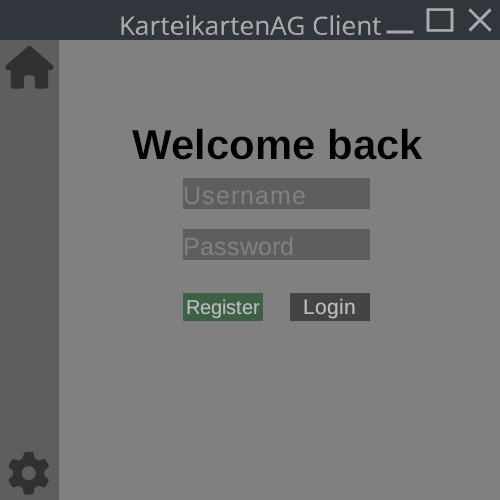
\includegraphics{images/login.jpg}
    } \\
    \noindent
    Von der Loginseite kann man ohne sich anzumelden \\ 
    bereits auf die Einstellungen zugreifen.

\end{answer}